\subsection{Traffic Patterns}
\label{cloud-measure-local}

\begin{figure}[!t]
\centering

%\minipage{0.31\textwidth}
\begin{subfigure}[b]{0.23\textwidth}
	\caption{HTTP flow count}
    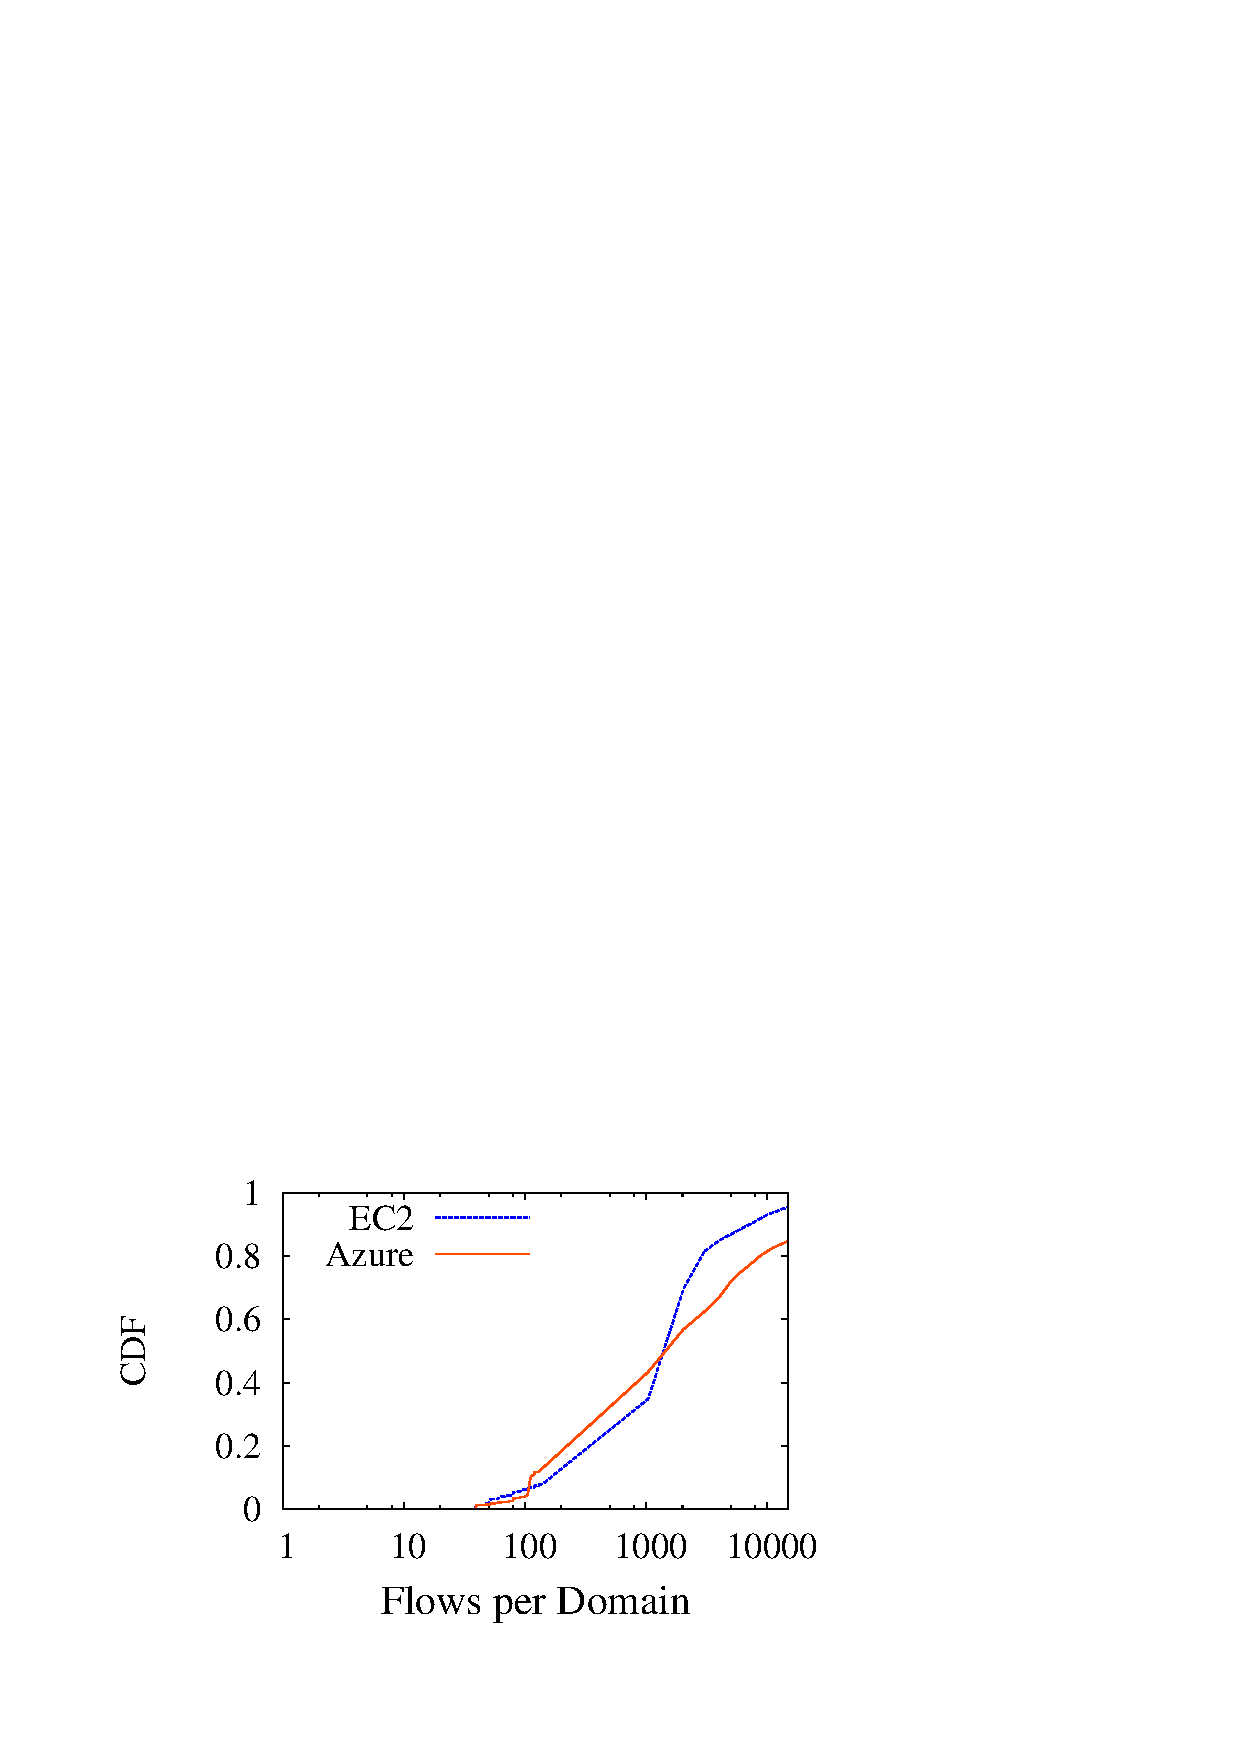
\includegraphics[width=\linewidth]{figures/cloudmeasure/imag_sec2/http_flow_cdf.pdf}
    \label{fig:httpflow-cdf}
\end{subfigure}
\begin{subfigure}[b]{0.23\textwidth}
    \caption{HTTPS flow count}
	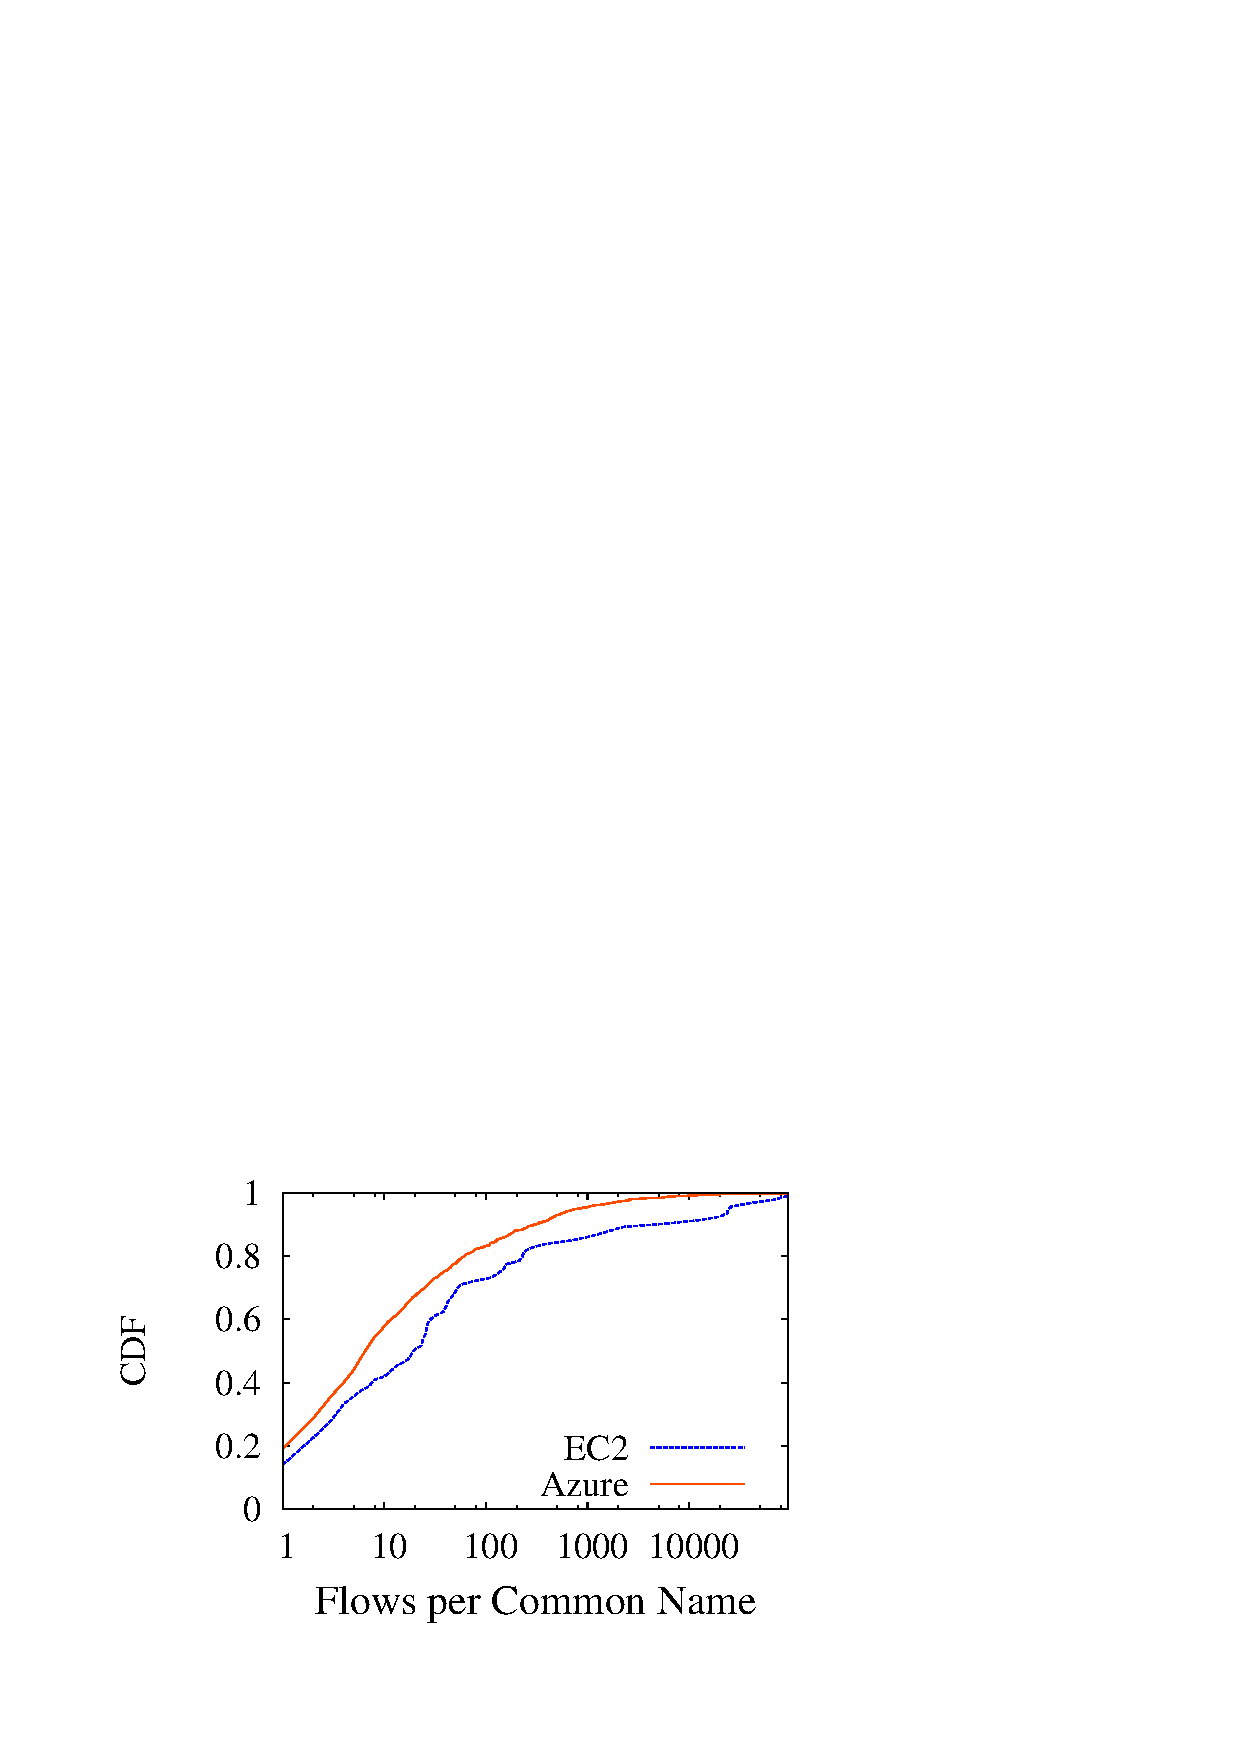
\includegraphics[width=\linewidth]{figures/cloudmeasure/imag_sec2/https_flow_cdf.pdf}
    \label{fig:httpsflow-cdf}
\end{subfigure}
\begin{subfigure}[b]{0.23\textwidth}
    \caption{HTTP flow size}
    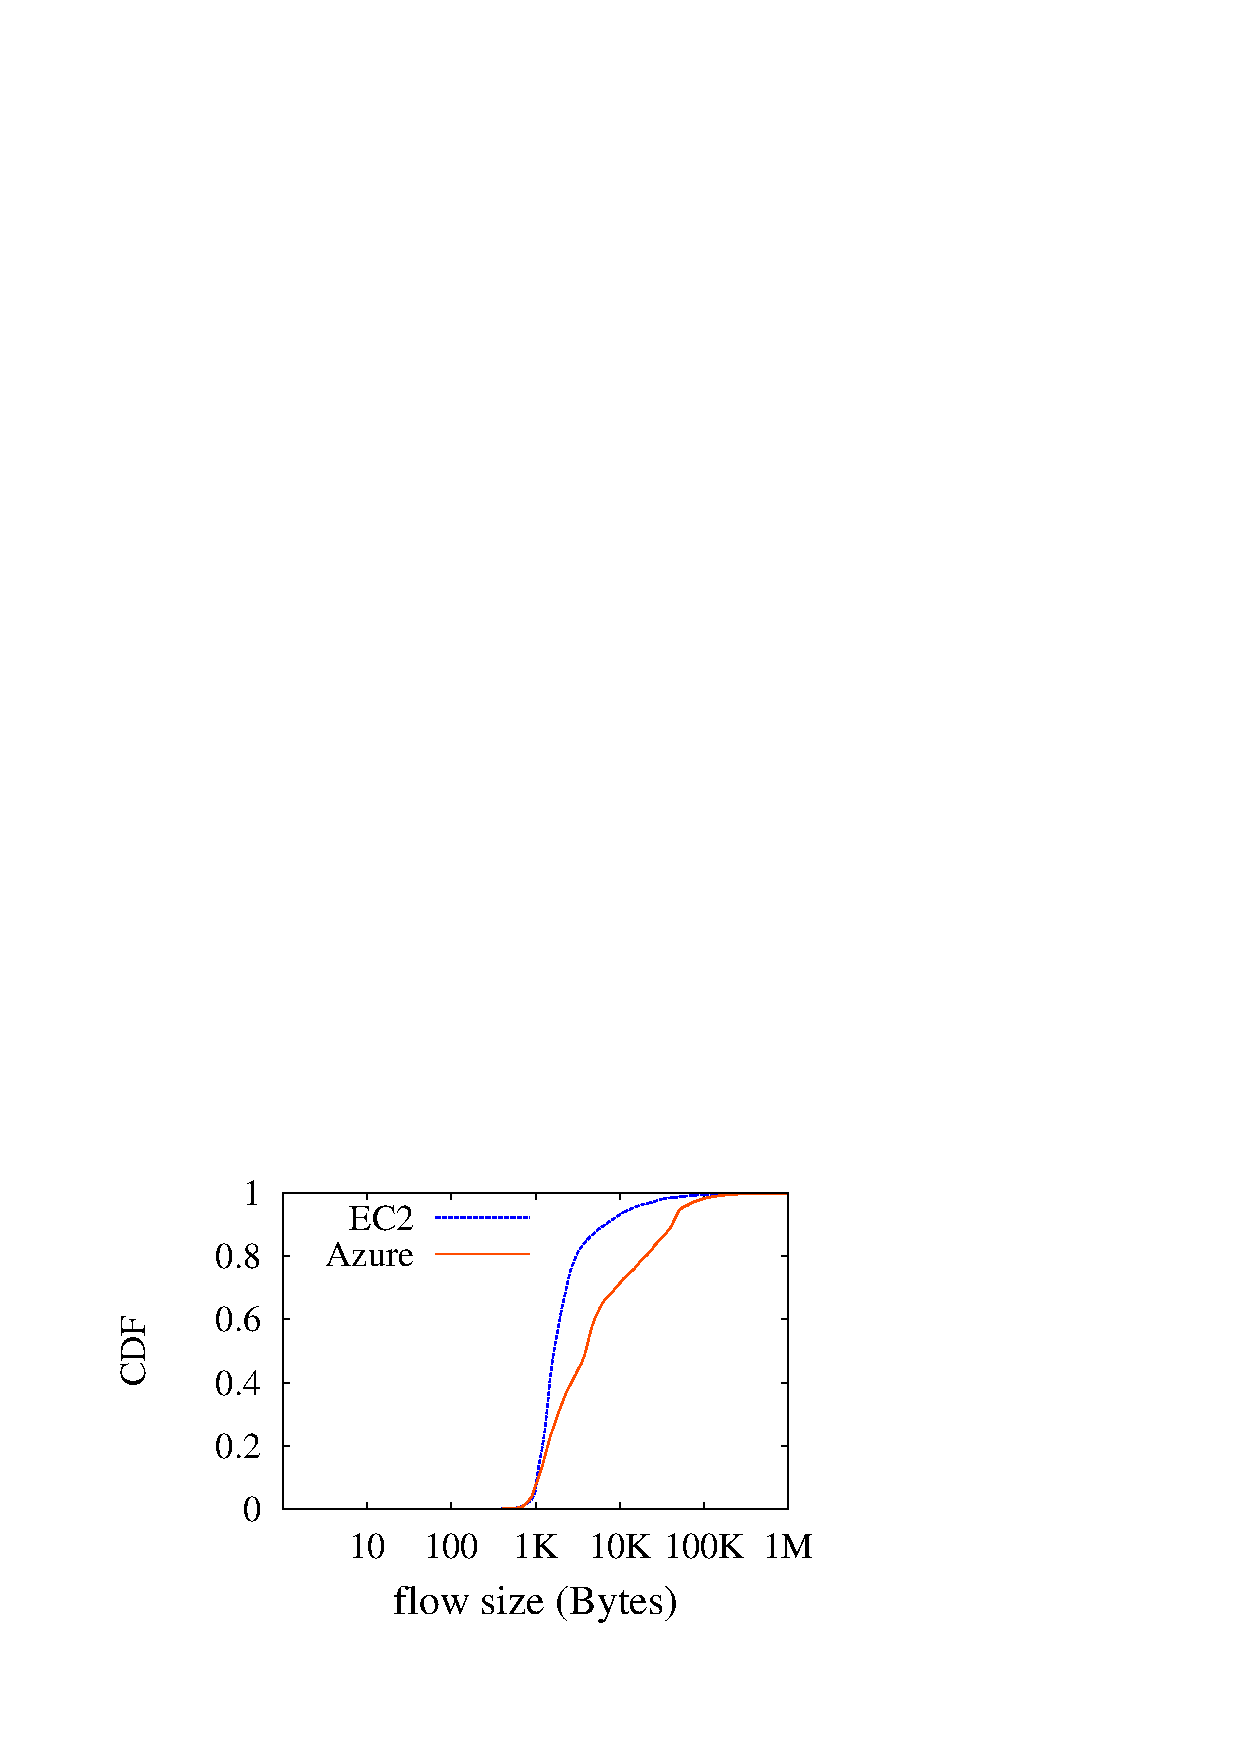
\includegraphics[width=\linewidth]{figures/cloudmeasure/imag_sec2/http_flow_size_cdf.pdf}
    \label{fig:http-flow-size-cdf}
\end{subfigure}
\begin{subfigure}[b]{0.23\textwidth}
    \caption{HTTPS flow size}    	
	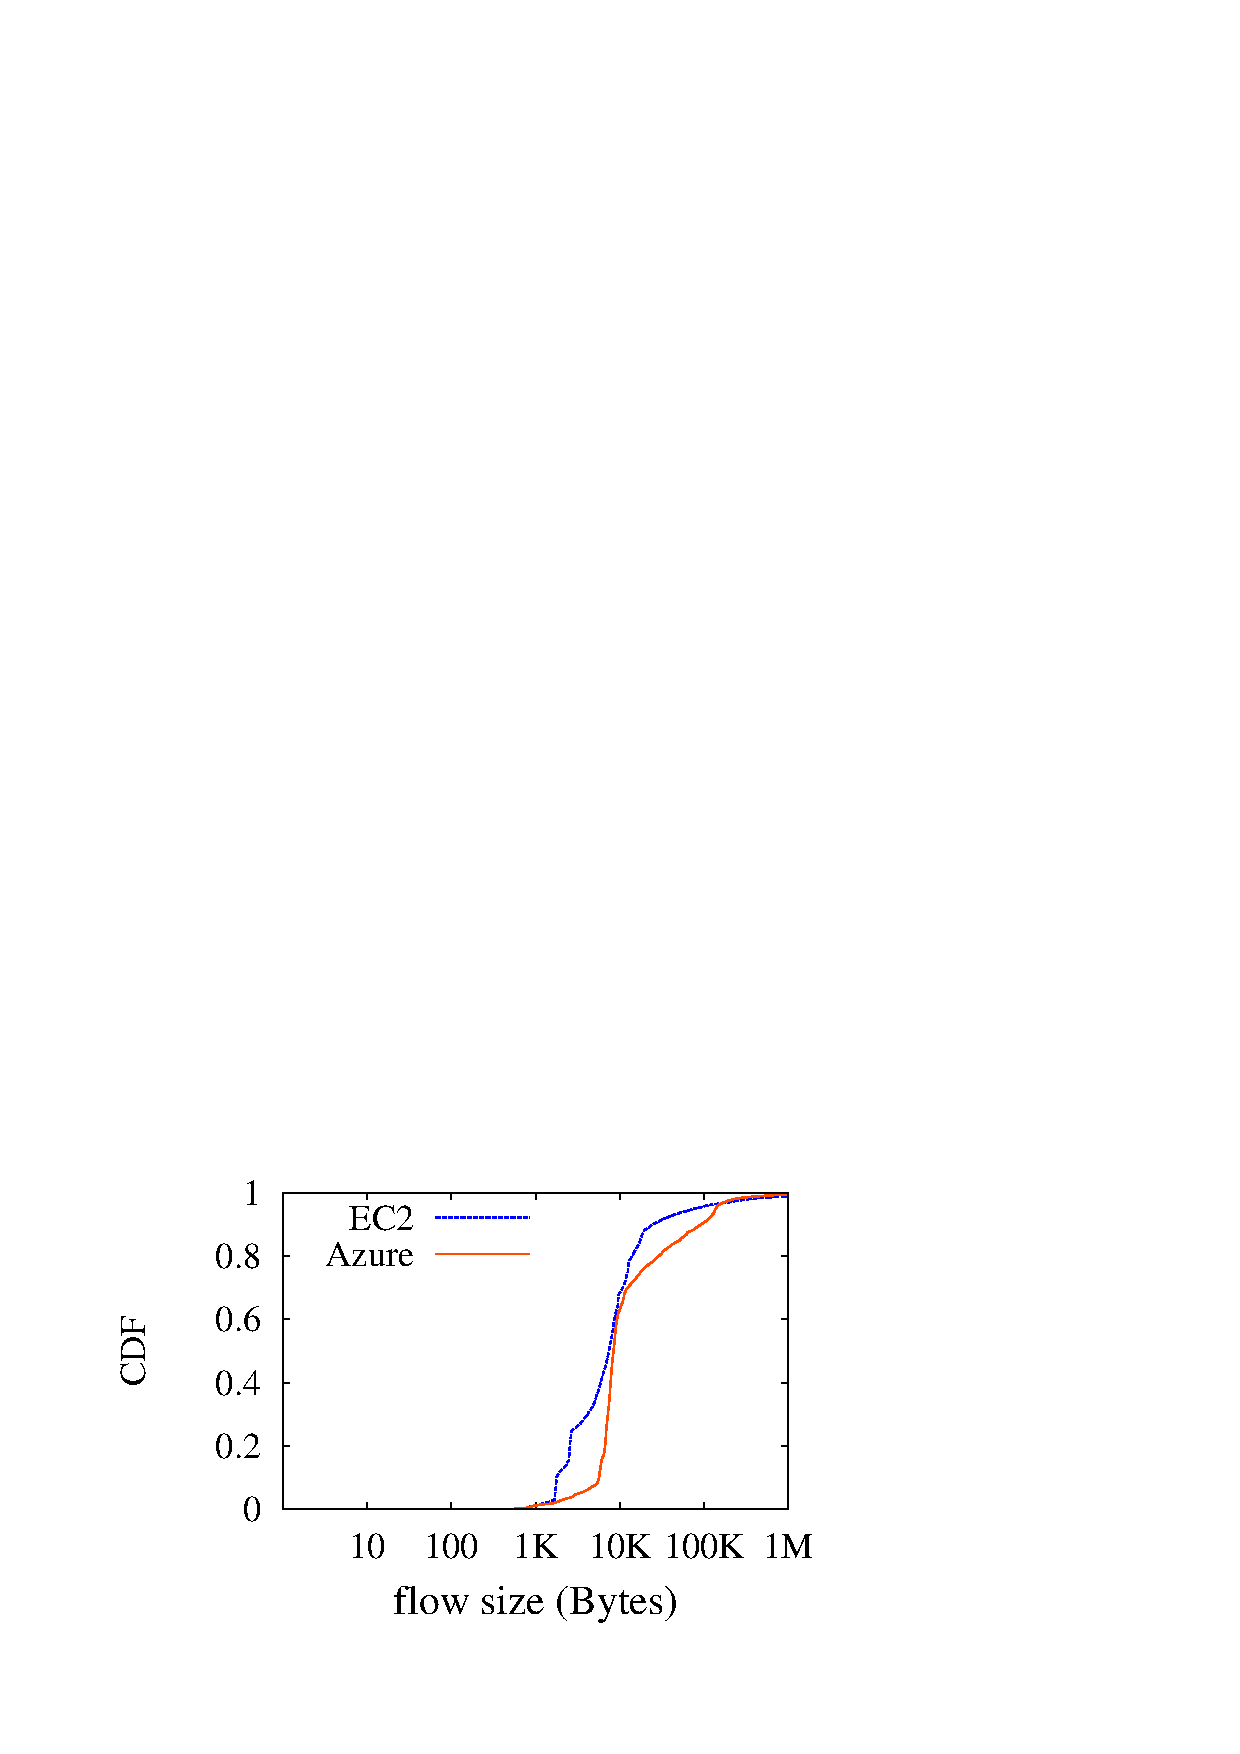
\includegraphics[width=\linewidth]{figures/cloudmeasure/imag_sec2/https_flow_size_cdf.pdf}
    \label{fig:https-flow-size-cdf}
\end{subfigure}

\caption{CDFs for HTTP/HTTPS flow counts and sizes.}
\label{fig:traffic-pattern}
\end{figure}


Our \captureonedata enables us to analyze not only who is running on the
cloud, but also the traffic patterns between clients in our university and 
cloud-resident web services.


\minisection{Flow-level properties} 
We first study the number of flows observed for various cloud-using domains 
in the \captureonedata. Figures~\ref{fig:httpflow-cdf} and
\ref{fig:httpsflow-cdf} show CDFs of the number of HTTP and HTTPS flows,
respectively, per-domain across our entire \captureonedata.  We observe that
$\approx$50\% of domains have fewer than 1,000 HTTP flows, and more than 80\%
of domains have fewer than 1,000 HTTPS flows.  Upon further analysis, we
found that the top 100 cloud-using domains are responsible for about 80\% of
the HTTP flows in EC2, and nearly 100\% of the HTTP flows in Azure; a long
tail follows for both clouds (CDF excluded for brevity). 

Flow sizes and durations generally appear to fit heavy-tailed
distributions (we omit durations in \figref{fig:traffic-pattern} for
brevity); similar properties have been observed for flows in other
networking contexts (e.g., in data
centers~\cite{benson2010network}). We note interesting differences
between HTTP and HTTPS: in particular, HTTPS flows are larger and last
longer than HTTP flows across both EC2 and Azure (e.g., median sizes
for EC2 are 10K and 2K, respectively).  This is expected given our
observation that a large percentage of HTTPS traffic is from file
storage services. In both cases, we see large flows that are more than a
few MB in size and long flows that last for a few hours.




